\chapter{Research Proposal}
\label{chap:proposal}

% feasible
% appropriate:  likely to deliver the evidence needed to answer the question
% rigorous
% likely to deliver valid, reliable, (generalisable?) results
% ethical
% justified


% \section{Justification} <-- already Chapter 2 and 3 contain it


% motivation
% Our goal is to provide a tool for doing framing analysis of multiple articles about a certain event, to highlight the different framing techniques and compare the resulting articles.
In this chapter, we present an overall description of the framework we want to build in order to highlight the different framing techniques and compare the articles that different sources create around a single event.
% This needs to be taken as a description of the requirements
% This description of the framework acts as a wireframe, where specific choices will be done based on evidence, 
As we can see in Figure~\ref{fig:diagram}, we are taking the research questions and sub-questions from the previous chapter, and for each one of them we have a process that from the hypothesis leads to some outputs using a separate and distinct analysis.

% outline
The structure of this chapter follows the vertical columns that represent the different research questions.

\begin{figure}[!htb]
    \centering
    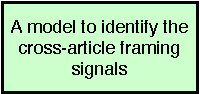
\includegraphics[width=\linewidth]{figures/diagram-RQ.pdf}
    \caption{The relationships between the research questions and the evaluations.}
    \label{fig:diagram}
\end{figure}

% Each one of the vertical columns is described in a different section below.

% This chapters begins with Section~\ref{sec:prop_pipeline} that outlines how we want to take existing works from the framing and similarity research areas.
% Then in Section~\ref{sec:prop_rq1} we target RQ1, giving some insights about some new analysis that we can do that would extend the existing automated framing analysis.
% And then in Section~\ref{sec:prop_rq2} we explain how we can analyse the role of news sources, for the relationship between their alignment and the framing they apply and how the stories are changed over time.



\section{Cross-article framing analysis (RQ1)}
\label{sec:prop_rq1}

% RQ1: framing differences
To address the first Research Question
\textbf{(How can we automatically reveal the framing differences in articles presenting the same event?)}, we aim to resolve the two sub-questions separately: the first one analyses the \textit{importance} of comparing multiple articles to understand the framing that is being applied on the news through the revelation of specific framing signals, and the second one explores \textit{how} we can build a tool to identify these framing signals automatically. The dependency between the two sub-questions underlines that the second column needs the outputs of the first one to have labels to attach to the framing differences.

% we aim to automatically identify \textit{signals of framing} that otherwise would not be noticeable: differences in emphasis and selection of details.
% These signals, while they are defined in the theoretical works, they have not been targeted in the automatic framing analysis.

% Starting with the \textit{emphasis}, we aim to analyse how different articles give importance to specific details.
% While existing works just focus on the usage of loaded terms and repetitions to indicate the presence of emphasis, we can enrich this analysis by seeing how other articles describe the same event.
% Comparing between different articles we can spot differences in the main focus of the article (e.g., the title is an indicator) or look at how the details are presented in a different order to set the priorities for the reader.
% And this can be combined with loaded language analysis, to see how certain details are emphasised and pushed with specific words in very different ways.
% \todo{figure}

% To understand the \textit{selection of details} instead, the idea is to compare the articles and get the common, unique and omitted pieces~\cite{bountouridis2018explaining} and then use some linguistic features (e.g., subjectivity, framing devices) to understand what is their role, may them be full sentences or just specific words that have been added or removed strategically.
% With this analysis, we aim to provide for each article, multiple sides of the same story with an insight into what changes between them.


\subsection{RQ1.1}
% RQ 1.1: cross-article signals
The first column represents an line of research that is needed to understand how useful is for readers to confront the information available in multiple articles to spot the framing techniques used.
% signals
In order to describe and characterise the framing we started from the literature review to gather concrete manifestations of framing, both in theoretical works and in detection methods.
As we have seen in subsection~\ref{ssec:lit_framing_theory}, different manifestations have been theorised and studied in practical studies
% what we mean by signal
We call these manifestation as \emph{signals} because they are signalling the presence of the framing, which is a abstract concept, but are tangible and can be seen as concrete features.
For example, loaded language can be seen as a signal that can be observed on specific words that have a strong sentiment, and evokes frames of strength, violence, threat and similar.
What we want to investigate is whether we can extend this set of signals by exiting the limitations of a single-article analysis. 
Our specific subquestion is \textbf{Which framing signals can be identified from the comparison of multiple articles?}

% Hypothesis
Our hypothesis is that all these signals will reveal far more than the single-article framing analysis.
We find that some framing signals just exist when we consider more than one article at a time, and have not been studied in automated detection methods.
We described them in a position paper~\cite{mensio2020towards} and defined as \emph{cross-article comparative signals}.

\todo{write a short abstract of the signals we expect to identify}
% % This is is the starting point to identify the differences, with a contrastive analysis. We propose here a set of  that can bring the narrative analysis a step further:
% \begin{itemize}
%     \item The \textbf{main focus} of the compared articles is on a different part or detail of the story: this means that while they are both describing the same broad event, they are trying to emphasise or prioritise two different aspects.
%     % Prioritisation is usually based on negativity / unexpectedness / superlativeness \cite{zahid2019towards}.
%     This signal can be computed by looking at the most similar sentence to the article title (proxy of the emphasis), and seeing how it is represented in other documents.
%     % Two articles that are semantically similar overall (they also have sentence-sentence pairs very similar) focus on different details when the titles are similar to different sentence-level cliques.
    
%     \item \textbf{Ordering}: the compared articles present the same details, but in a different order.
%     Re-ordering events tends to be an efficient way of creating implicit cause-effect relationships. 
%     To do this comparison, it is sufficient to find the crossovers in the sentence-level connections.

%     \item \textbf{Selection of details}:
%     One article is \emph{omitting} certain details that have been reported by other articles, or is describing events that are \emph{corroborated} by other sources, or has \emph{unique parts} that do not occur in other articles~\cite{bountouridis2018explaining}.
%     In addition to seeing which parts are selected or omitted, the narrative analysis can help us to find some insights about them (e.g., the article is omitting subjective statements reported by others, or is describing a background event that others did not include).
%     % For the detection of this case, we rely on the work~\cite{bountouridis2018explaining}.
    
%     \item The articles are \textbf{framing} the narrative in different ways from each other. This manifests through comparing linked sentences to observe the differences in terms of framing features: the considered articles are describing the same events but with different framing and reasoning.
%     One concrete example is the usage of \emph{causality}: one article may contain causality signposting between a pair of sentences that is absent elsewhere.
%     % \item The article uses \textbf{causality as a weapon} (where there is no proof of causality).
%     % An article is expressing causality when there are certain devices (signposting) between two sentences/events.
%     % Different articles may show the causality with different levels, so one sees it as causal and the other one does not link the events.
%     Or as another example, the usage of \emph{specific words} can reveal a specific framing: talking about the same detail or entity, the usage of verbs or adjectives may change.
%     % find strong sentiment and subjective words 
%     % (as adjectives for the same entity, or as verbs).
%     % Detail (e.g. black man instead of just saying man, to add a subtle bias).
%     For detecting such peculiarities, %and comparing them, we can combine the framing signals with 
%     features as Named Entities and subjectivity may be combined.
%     % use features coming from subjective and sentiment analysis.

%     \item The comparison can be also done on the \textbf{subjectivity} of the article: both at the document level (saying that this is an opinion piece, while a similar one is more factual) or at the sentence level, by interweaving this signal with the ones proposed before.
%     % is a \textbf{mix of factual and opinionated / subjective} content: subjectivity values on the full document and on specific sentences.
%     % A sentence is on one article subjective and a similar one on a different article is objective.
%     % Also look at the role of the sentence (commentary, action, background). 

% \end{itemize}

% From the signals in Figure~\ref{fig:comparison}, we can see that the first article pushes the narrative towards \texttt{risk} and other negative frames, to sustain the idea presented in the title ``Britain on Edge''.
% The second article, even though it has a lot of information in common with the first one, is more confident on the preparedness of the National Health Service to face the virus (e.g., \texttt{confidence}, \texttt{expertise}).
% The extraction of these cross-article signals is the first step to finding possible cases of manipulation.

% The expansion and refinement of these signals will help us answer RQ1.1.


% requirements
In order to validate our hypothesis, we will run a \textbf{user study} where participants will be presented with different short texts that present differences.
% data (hand-picked samples from sources with different political alignment)
This data will come from a small set of samples made of pairs of documents that are presenting the same detail, with some differences in the terms used. To collect this data we will use articles that are already clustered as discussing the same specific event (from AllSides and other news aggregators like Google News).

% analysis
Participants will be presented with two articles and will be asked a set of questions that investigate the effect of having different terms, different details and how user think this is related to try to push for a certain perspective on the events described.
% Do the articles have the same point of view? Do they convey the same message? Title? Details?
% Sentences
% - Do these sentences have different information?
% - Do they provide different perspective?
% - Are there any terms that push for a certain perspective?
% - What is the difference in the intent of communication?
%   - Detail (random, look like professional and detailed, mislead, emphasise on something)
%   - Word choice: emphasise, promote, demote
% if they value the selected differences as signals of the different point of view of the sources (framing), and what they think that the difference is (is it that they are omitting something, commenting, emphasising, other)?

Or study 2 (better):
To test the hypothesis that framing is easier to spot when multiple articles are presented. First present to the user just one article and ask to find the framing signals. Then show second article with different details and ask again.
It is important to divide the annotators of a certain pair in two subgrups in order to divide the effect of ``seeing again the same article twice'' from ``seeing the article compared to another one''. For this reason, if we consider A1 and A2, user U1 will first see A1 then A1+A2, while U2 will first see A2 then A1+A2. In this way we can sum CA1\_before+CA2 for U1 and CA1+CA2\_before for U2 where each observation is done at first sight of the article (see Figure).
Hypothesis: users will be able to see more signals in the second phase.

\begin{figure}[!htb]
    \centering
    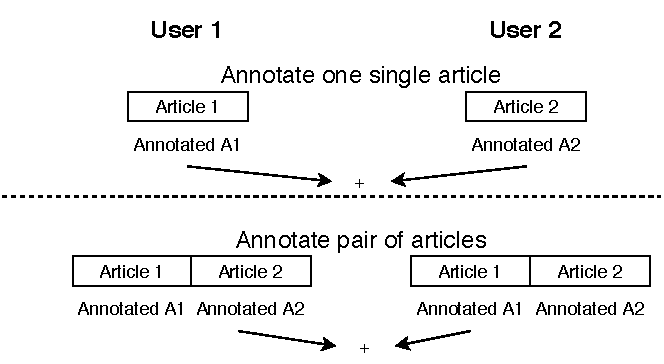
\includegraphics[width=\linewidth]{figures/diagram-user-study-flow.pdf}
    \caption{How to compare the user annotations to exclude effects of second-reading}
    \label{fig:user-study}
\end{figure}

The data required from the user is to highlight parts of the article(s) and to say why it is providing a certain view angle, as a free text. Suggesting some techniques from literature.

% outputs
The annotations will be manually examined with two goals.
First, to see if the annotators (using inter-annotator agreement measures) are able to spot more signals with different articles in their front.
This will prove or disprove our hypothesis that framing can be revealed easier with multiple articles.
And second the annotations will be classified manually to bring them back to some categories that represent framing signals. An example could be ``omission of opposing detail'' or ``biased term''. We need to come up with a set of labels that we can assign to the differences pointed out by the users.


\todo{what about an figure/example of the task?}


\subsection{RQ1.2}
% how would a cross-article framing analysis perform

The second part of the first RQ requires building and evaluating an automated method to extract the signals identified.
\textbf{To what extent can an automated framework recognise framing signals?}

% implementation
Taking the outputs of the first study, we will create a processing pipeline with strategies to identify the framing signals. This will involve reasoning over the features already provided by the pipeline and building a model that provides as outputs span annotations of framing that will say which framing technique has been used.

% dataset building
In order to evaluate the baseline built, we will need to collect a larger \textbf{dataset} than the User Study 1, where manual annotators will be given the task description and will annotate the document pairs (help of pipeline to provide similar articles and candidate sentences).
This dataset will be made available as a resource paper.

% evaluation
The baseline will be evaluated by looking at the accuracy/precision/recall of the span pairs that contain framing differences compared to the gold standard

% outputs
The output of this research will be a tool that shows the framing differences between news articles.

Once the tool has shown enough accuracy, we plan to put it in an online setting where people will continue correcting the outputs and provide more training data.

\subsubsection{Processing Pipeline}\todo{remove? does it make sense? 4.1.2}
\label{sec:prop_pipeline}
The first objective is to build a representation that describes how the articles, and parts of them, are related between each other, together with the framing features coming from the single-article analysis.

This is the starting point that is required to do all the expansions investigated by the research questions.
Even though there are multiple works on automated framing analysis, the implementations are sparse and mostly focused on specific topics.
Here instead we want to have a generic pipeline that would work for any topic.
???

This pipeline

\begin{figure}[!htb]
    \centering
    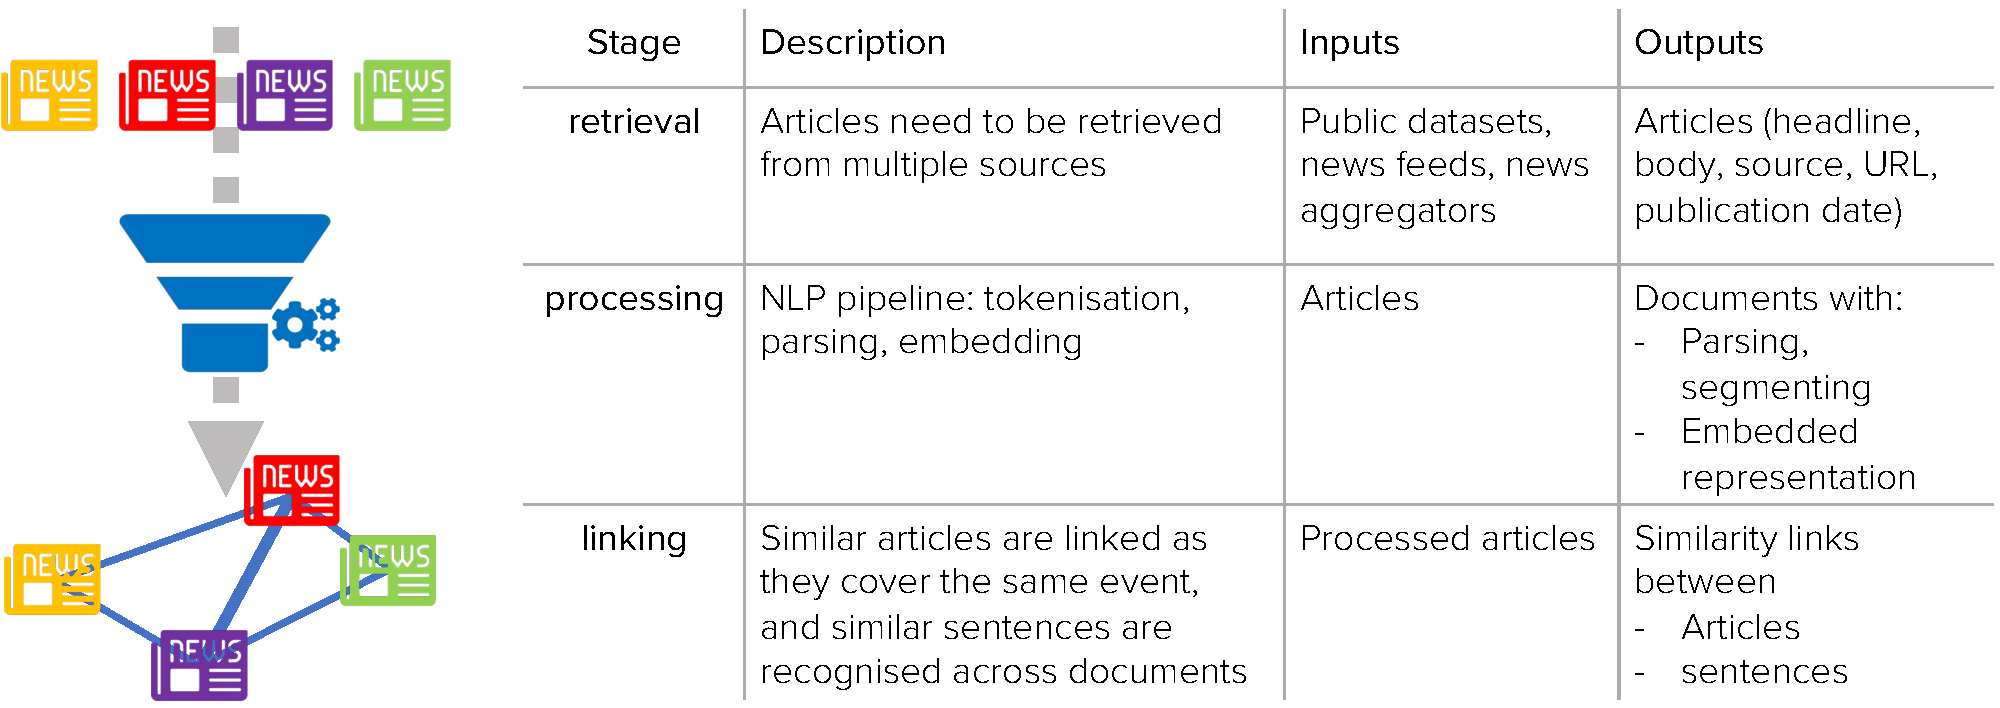
\includegraphics[width=\textwidth]{figures/figure_pipeline.pdf}
    \caption{The processing pipeline that retrieves, processes and links together different articles.}
    \label{fig:pipeline}
\end{figure}

As we can see in Figure~\ref{fig:pipeline}, the processing pipeline is made of different stages:
% The processing pipeline we propose for this purpose is made of multiple steps:
\begin{itemize}
    \item \textbf{preprocessing}: documents are retrieved, cleaned up and fragmented into paragraphs and sentences;
    \item \textbf{narrative features} are attached to each document, paragraph and sentence belonging to three main types:
    \emph{structural role} using and highlighting the linguistic devices provided by~\cite{zahid2019towards};
    \emph{framing features} are extracted (framing and reasoning devices) finding some linguistic representatives from~\cite{gamson1989media,fillmore2006frame};
    \emph{subjectivity} is computed, and strong word choices are highlighted~\cite{liu2010sentiment};\todo{expand on single-article framing signals}
    \item \textbf{linking}: \emph{similar articles} are found by using document-level similarity measures: in this way it would be possible to find groups of documents that describe the same events; \emph{similar sentences and paragraphs} are found by sentence-level similarity measures, inside each group of documents: corroborated and omitted sentences are identified~\cite{bountouridis2018explaining}.
\end{itemize}
% We start with an example of analysis together with the processing pipeline, % that enables this and 
% then we introduce some cross-article signals that highlight the difference in the narratives used.
% First we describe how we think is more reasonable to process the documents (similarity, cliques, hierarchical topic/stories).
% Then we describe which are the  (baseline)(with list).

At the end of the pipeline, we will have available a representation for the articles that accounts for how they are similar on the document level and at the sentence level.
% also single-article framing features
This representation would allow us to navigate between different articles and see their features. We will exploit this representation for answering the two Research Questions, as shown in the following sections.


\section{The role of news sources (RQ2)}
\label{sec:prop_rq2}
% RQ2: also the sources

The purpose of the second research question is to understand the link between news sources features and how they frame it, changing details and taking information from other sources.

While the first research question focused on how to reveal the framing, here we want to investigate how the sources interact with framing. For this purpose, we have two subquestions that investigate \emph{i)} the relationships between the affiliation of a source and the framing that it uses, and \emph{ii)} how stories are modified and reframed over time when sources reuse contents from other articles.

\subsection{RQ2.1}
% RQ2.1: relationship with source information
\textbf{How does the affiliation of a news source relate with the  framing techniques it uses?}
We want to analyse the relationships between the framing choices done by the authors and the news sources where the articles are published. In other words, we want to understand the relationships between the ideological alignment of the news outlets (political alignment, bias, newsgroups) and the effective differences contained in the articles.

Data requirements: info for each source



% {RQ2.1: How well does the framing analysis relate with the information available on affiliation, newsgroup and bias of the single outlets?} With different features available for news sources, we want to see if some of them are related to the amount and type of framing that occurs on their articles.

With RQ2.1 we ask how does the framing analysis relate with the information of the single outlets (affiliation, newsgroup, bias, partisanship, ...).

% Hypothesis

% requirement: data on news outlets
This question can be answered by pulling together information about news outlets.

- MBFC: political bias and factuality

- newsgroup: search info

- geography: country, region

- Others?

% how to answer RQ?
And once this information is available, we can aggregate a set of framing features (to be defined!!!) by the source of the articles.

With these two groups of information, we can study their correlation.

% possible outcomes
What a correlation analysis may say? For example that sources heavily biased (score on the source) tend to perform omissions or use loaded language.


% significance


\subsection{RQ2.2}
% RQ2.2
\textbf{To what extent can we identify the evolution of the framing of a certain event?}
And if we also take the timing information (publication time), we can expand this model to characterise the evolution of information, describing how different news sources reuse contents from others and how the details are selected and changed over time.
In this way we aim to extract \textit{information flows}, showing over time how different sources treat different details of the events, evolving the narrative, acquiring new elements from other sources and dropping other information pieces.\textbf{}

Data requirements: timing information.
Is it reliable? How to manage intervals and not only instants





% \section{Possible outputs}


% Tool for finding other stories on the same event
% External facts not considered
% Highlight words that are used differently
% Tool to analyse the practices of news outlets
% From where do they get info
% How they change it
